\chapter{Experiments}

The main purpose of the experiments executed for this work is to provide a comparison with the paper \cite{LingZhen2021Sbtb} discussed in the background section about remote attestation using ARM TrustZone. To be able to compare the results of this work and that of the paper the experiments need to be made as similar as possible which will be clearly visible. Secondly for the security evaluation the solution of this work will be evaluated and the differences with the security evaluation of the paper will be highlighted.

\section{Performance}

\paragraph*{}%{Trusted boot}
The trusted boot experiment in the paper is based on the attestation of the normal world before giving it control. In the paper they talk about 107 MB of file system image that is being measured in 1.276 seconds so this could be a valuable starting point to compare their performance with the performance achieved in this thesis. Because the implementation of this work is focused on measuring code pages there will be a difference in what is measured. While it can be somewhat assumed that the memory space of the file system in the paper is contiguous or at least the mapping can be found rather easily, the code pages in the implementation of this work are spread across multiple processes which need to be considered one by one. Looking up the right memory pages to measure them incurs additional overhead which needs to be taken into account, that is why we opted for three different experiments that relate to this trusted boot experiment from the paper. One experiment will measure all the code pages of all the processes in the simulation, the second one will measure all code pages of one process and the last experiment will measure one contiguous memory region of code pages from one process.

\paragraph*{}%{Overhead}
The overhead of running the attestation module is measured in the paper by executing system services from the Linux kernel and running this experiment with and without the attestation module being active. The results in the paper of this experiment were overhead between $- 0.55 \%$ and $+ 0.67 \%$ on different system calls. These results don't give much insight in the matter in our opinion because some key information is missing to correctly assess the results. First of all it is not mentioned how often the attestation is running while these system calls are made. Secondly it can be assumed that the attestation does not get priority over the system calls but this is also not explicitly mentioned. Last but not least, the range of $- 0.55 \%$ and $+ 0.67 \%$ doesn't really tell much, this could just be standard deviation. For this experiment it was not mentioned how often it was executed which gives the impression that this is a one time measurement. They are however explicit about calling each service 1000 times, with intervals of 250 ms between each call and they do this with 7 different system services, which as they also include adds up to almost 30 minutes.

\section{Performance Evaluation}

\paragraph*{}%{All processes}
The total amount of loaded code pages in RAM is around 1850, the time it takes to measure those twice (once for initialization and once for attestation) is about 25 seconds. A plot is shown which provides the experiment being executed 10 times, also a linear regression line can be found to provide the general correlation between the amount of pages measured and the time it takes.

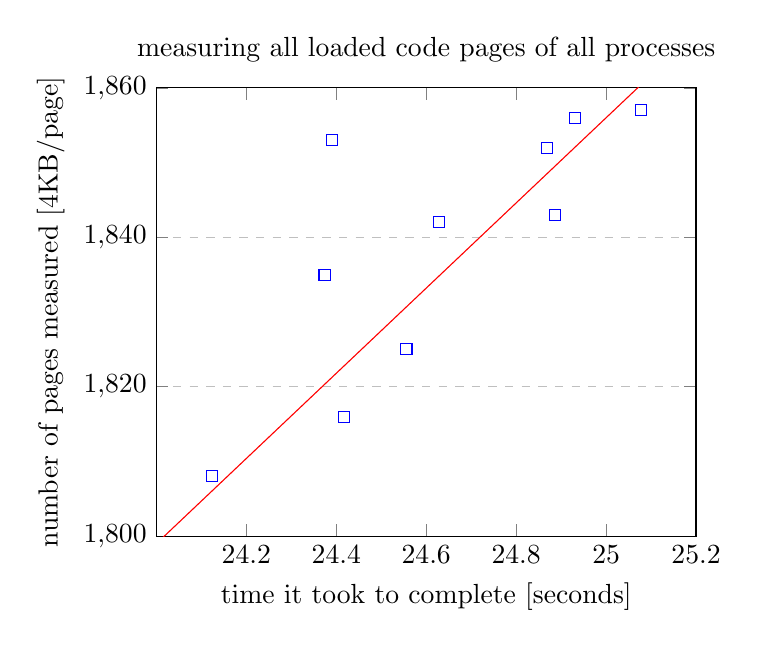
\begin{tikzpicture}
\begin{axis}[
    title={measuring all loaded code pages of all processes},
    xlabel={time it took to complete [seconds]},
    ylabel={number of pages measured [4KB/page]},
    xmin=24, xmax=25.2,
    ymin=1800, ymax=1860,
    xtick={24.2,24.4,24.6,24.8,25,25.2},
    ytick={1800,1820,1840,1860},
    legend pos=north west,
    ymajorgrids=true,
    grid style=dashed,
]

\addplot [
    domain=24:25.2, 
    samples=100, 
    color=red,
]{57*x + 431};

\addplot[
	only marks,
    color=blue,
    mark=square,
    ]
    coordinates {
    (24.868,1852)(24.886,1843)(24.556,1825)(24.930,1856)(24.390,1853)(24.123,1808)(24.417,1816)(24.629,1842)(25.078,1857)(24.374,1835)
    };
    
\end{axis}
\end{tikzpicture}

\paragraph*{}%{One proces}
To provide insight in how long it takes to measure one process (twice) we executed the last experiment on just the \textit{init\_proc} process.

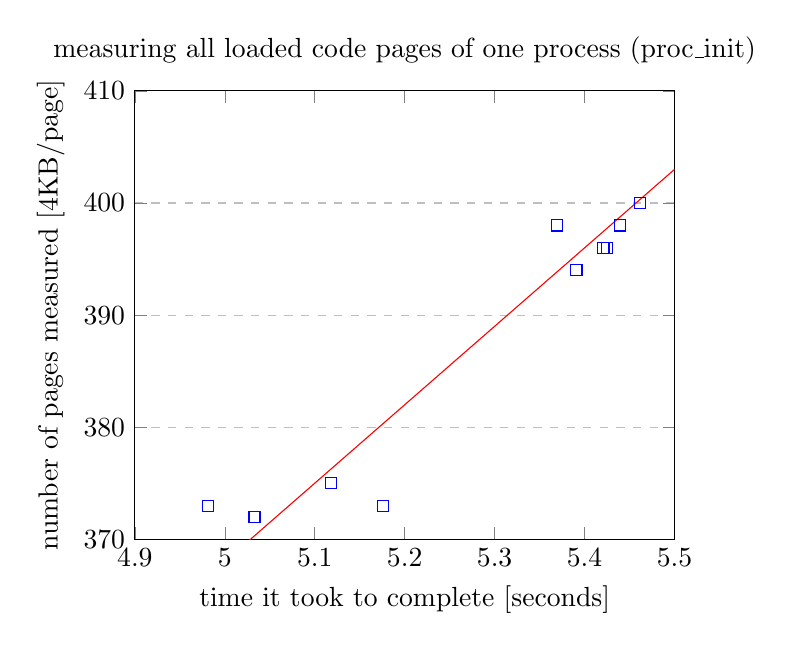
\begin{tikzpicture}
\begin{axis}[
    title={measuring all loaded code pages of one process (proc\_init)},
    xlabel={time it took to complete [seconds]},
    ylabel={number of pages measured [4KB/page]},
    xmin=4.9, xmax=5.5,
    ymin=370, ymax=410,
    xtick={4.9,5,5.1,5.2,5.3,5.4,5.5},
    ytick={370,380,390,400,410},
    legend pos=north west,
    ymajorgrids=true,
    grid style=dashed,
]

\addplot [
    domain=4.9:5.5, 
    samples=100, 
    color=red,
]{70*x + 18};

\addplot[
	only marks,
    color=blue,
    mark=square,
    ]
    coordinates {
    (4.981,373)(5.421,396)(5.369,398)(5.462,400)(5.391,394)(5.033,372)(5.439,398)(5.425,396)(5.118,375)(5.176,373)
    };
    
\end{axis}
\end{tikzpicture}

\paragraph*{}%{One memory region}
In the first two experiments the amount of pages that are loaded into RAM fluctuated a bit, this probably has to do with pages being swapped in and out of memory. In this last experiment only one executable memory region of the \textit{init\_proc} is measured and the amount of pages stays constant for all 10 iterations. The amount of pages measured is 88 and the average execution time is 1.319 seconds, the maximum execution time is 1.353 and the minimum 1.299.

\paragraph*{}
Last but not least the three experiments are plotted in one graph to show how they relate to each other. This plot clearly shows that the amount of time the measurements take is proportional to the amount of pages that are measured. No surprises here because hashing the memory pages is the most compute intensive task of the program but it is good to compare between the different experiments nonetheless. This allows us to compare our achieved performance to that of the paper because we can extrapolate the results to the necessary amount that was measured in the paper.

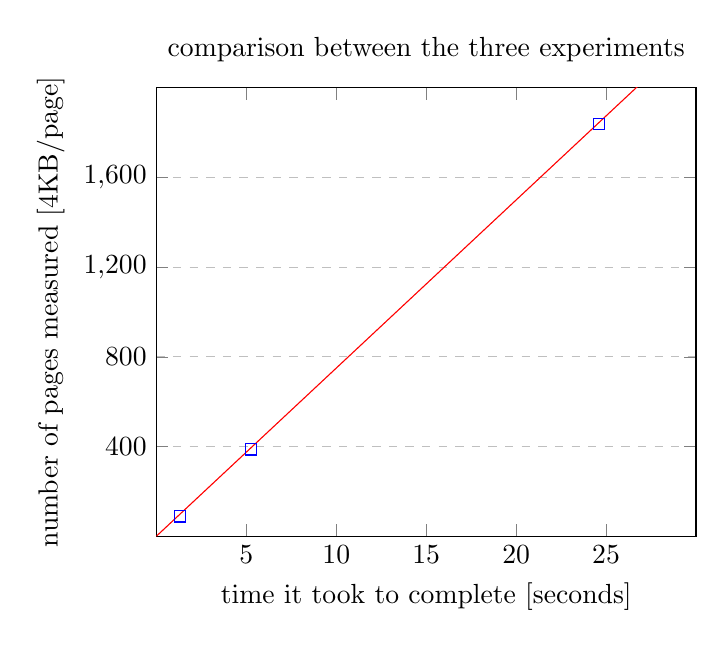
\begin{tikzpicture}
\begin{axis}[
    title={comparison between the three experiments},
    xlabel={time it took to complete [seconds]},
    ylabel={number of pages measured [4KB/page]},
    xmin=0, xmax=30,
    ymin=0, ymax=2000,
    xtick={5,10,15,20,25},
    ytick={400,800,1200,1600},
    legend pos=north west,
    ymajorgrids=true,
    grid style=dashed,
]

\addplot [
    domain=0:30, 
    samples=100, 
    color=red,
]{75*x};

\addplot[
	only marks,
    color=blue,
    mark=square,
    ]
    coordinates {
    (24.625,1839)(5.281,387)(1.319,88)
    };
    
\end{axis}
\end{tikzpicture}

\paragraph*{}%{Comparison}
As can be seen in the three executed experiments, the performance of the implementation of this work is far from that of the paper. Certain aspects are important to highlight which give a partial explanation about the cause of these deviations. First of all the implementation is not written nor fine tuned for performance, it is merely written as a proof of concept. This is due to the restricted amount of time and the lack of experience with making software with high performance. Secondly the memory regions that are attested in this work are only the executable memory pages of a process. These pages need to be identified using multiple files which generally takes more time than in the case that there is one large chunk of memory that is attested. Lastly these experiments are executed on a Qemu emulation of OP-TEE on a general purpose laptop (Lenovo Thinkpad P50) while the experiments in the paper are executed using a hardware prototype. 

\paragraph*{}%{Balance}
While it is hard to make any conclusions based on these pessimistic results, it is useful to elaborate about the balance between performance and added security. A good balance between performance overhead and security assurance depends on the use case. In case of a smart phone we believe even with these results that attesting the executable pages that are loaded in RAM memory every 30 minutes has not too much impact on the user experience. Depending on the amount of newly loaded memory pages when an application is started it could even be considered to attest these pages before starting to execute them. This is a lot more sensitive towards the user experience because this happens while the user is waiting for the application to open, while on the other hand running the attestation in the background on the already loaded pages in RAM should have minimal impact on the user. These considerations do not take into account the energy consumption of running the attestation, because we didn't have the means for these kinds of experiments.

\section{Security Properties}

\paragraph*{}%{}
The attestation method presented in this work focuses on measuring the code pages of processes loaded in RAM. A code page can only gain control or be executed when it is loaded in RAM first. Keeping this prerequisite in mind it should suffice to only attest those pages to ensure no code page that has been tampered with gets to be executed. This last statement of course needs to be loosened a bit because the attestation runs periodically so a code page may have been executed before the changes are noticed by the attestation PTA.

\paragraph*{}%{Integrity of the measurement execution}
Integrity of the measurement execution is of utmost importance when it comes to attestation. In remote attestation the critical code runs on a hardened server which guarantees that it is infeasible to tamper with the execution control flow. In the case of the PinePhone it is not remote attestation we present but user attestation, the critical code which compares the measurements runs in the Secure World. The Trusted Execution Environment provided by ARM TrustZone does guarantee that the Normal World cannot influence the execution of the Secure World in any way as long as the device was started up successfully using secure boot.

\paragraph*{}%{Secure storage of results}
Secure storage of results is very important to have a chance at making remote attestation work. If an adversary were to be able to tamper with these values they could make every attestation attempt fail due to the changed initial value. In case a bad hashing algorithm is chosen and the attacker is able to read the initial hash digest they could also try to forge a collision attack where they tamper with a page in such a way that it's hash digest doesn't change but the code in the page does something the attacker desires. To make sure the reference values are not tampered with they need to be stored in secure memory which should not be accessible from outside the secure world. In the secure world these values should only be written during the initialization phase and afterwards only read. This statement can again be loosened a bit in case there are software updates or additional software to be installed on the device. The initialization phase could be executed again for those code pages and updating or adding the measurement results to the secure storage. 

\section{Security Evaluation}

\paragraph*{}%{Security guarantees}
Security guarantees that can be made are the integrity of the measurement execution control flow and the integrity and confidentiality of the results that are being stored. These are achieved due to secure boot enabling the trusted execution environment of ARM TrustZone. These are key assumptions in the field of remote attestation and thus are also very important in this case of user attestation. Of course when discussing the security guarantees a certain solution offers it is not only about the execution and storage of that application itself but also what additional security guarantees it provides to the system overall. The most important guarantee that an attestation solution tries to provide is being able to detect modifications or unexpected possibly malicious changes to the aspects of the system it attests. In our case the code pages of processes are being attested, we only measure the ones that are present in RAM because only then they are able to do harm to the system. There is still an unsolved problem as also stated in the paper that the rich OS needs to provide the physical addresses of the code pages. This means that malware capable of self hiding or transient root kits are still possible threats that could stay unnoticed to this solution. If an adversary has taken control of the OS there are countless ways in which the attacker could deny the attestation PTA the necessary addresses which at this moment would not result in an attestation alert to the user.

\paragraph*{}%{Shortcomings}
OS/firmware attacks are present in the attacker model of the paper on which this work is based. We believe that with this method the code pages of all processes including those of the rich OS can be attested and this will enable the user to be notified about any tampering with this code base. This does not mean however that tampering with these code pages has become harder and besides tampering with code there are lots of different methods to perform an OS/firmware attack. We believe that this work can be extended upon to thoroughly attest the Normal World (user applications and rich OS) but in it's current state it only allows detection of a small portion of the possible OS/firmware attacks. Even with the problem that the rich OS provides the physical memory addresses solved this incompleteness persists.

\paragraph*{}%{Extensions}
The paper also seems to claim that software attacks are protected against or detectable in the case of attestation. Again in this case we do not think this is a valid statement because the integrity of the code is only a small portion of the attack surface. In this attestation method the data structures are not checked which are the main target for very well known attacks that have been around for decades like buffer overflows and return oriented programming. Extensions to this solution need to be realized to detect software attacks, OS/firmware attacks likewise.